
\section{Experimento BRDF Edwards 2006}
\label{section-experiment-edwards-2006}

No artigo de Edwards et al. \cite{edwards2006halfway}, é apresentado o conceito do \textit{Halfway Vector Disk} como uma extensão para modelagem de BRDFs. Este método, usado neste experimento, propõe uma abordagem geométrica que melhora a eficiência computacional. As equações principais são descritas na \autoref{fig-edwards-2006-eqlang-latex}, com o código fonte em \texttt{EquationLang} disponível no \autoref{cod-edwards-2006-eqlang}. Os códigos gerados em GLSL podem ser vistos no \autoref{cod-edwards-2006-glsl-pt-1} e no \autoref{cod-edwards-2006-glsl-pt-2}. A renderização de objetos 3D utilizando o método pode ser observada na \autoref{fig-edwards-2006-eqlang}, enquanto os \textit{plots} estão ilustrados na \autoref{fig-edwards-2006-plots}.

%%%%%%%%%%%%%%%%%%%%%%%%%%%%%%%%%%%%%%%%%%%%%%%%%
\subsection{Representação em documento \LaTeX{}}
%%%%%%%%%%%%%%%%%%%%%%%%%%%%%%%%%%%%%%%%%%%%%%%%%
\begin{figure}[H]
    \caption{\label{fig-edwards-2006-eqlang-latex} \small Equações da BRDF do experimento Edwards em documento \LaTeX{}.}
    \begin{center}
        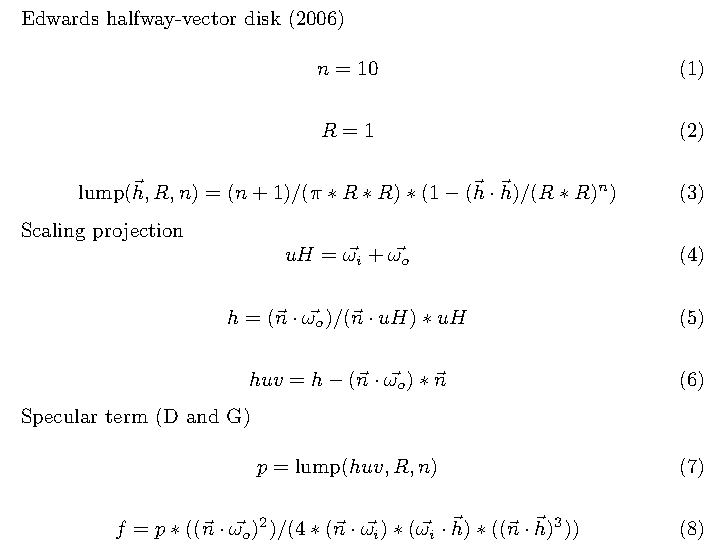
\includegraphics[scale=0.92]{./Imagens/brdfs/edwards-2006.pdf}
    \end{center}
\end{figure}

%%%%%%%%%%%%%%%%%%%%%%%%%%%%%%%%%%%%%%%%%%%%%%%%%
\subsection{Código GLSL Gerado}
%%%%%%%%%%%%%%%%%%%%%%%%%%%%%%%%%%%%%%%%%%%%%%%%%
\begin{codigo}[H]
    \caption{\small Saída do compilador: código GLSL da BRDF do experimento Edwards (parte 1 de 2).}
    \label{cod-edwards-2006-glsl-pt-1}
\begin{lstlisting}[language=C, inputencoding=utf8]
analytic ::begin parameters
#[type][name][min val][max val][default val]
::end parameters
::begin shader
//////////// START OF BUILTINS DECLARTION ////////////
vec3 var_0_vec_h;
vec3 var_3_vec_n;
float var_10_theta_h;
float var_11_theta_d;
float var_1_pi;
float var_2_epsilon;
vec3 var_4_vec_omega_i;
float var_5_theta_i;
float var_6_phi_i;
vec3 var_7_vec_omega_o;
float var_8_theta_o;
float var_9_phi_o;
//////////// END OF BUILTINS DECLARTION ////////////

//////////// START OF USER DECLARED ////////////
vec3 var_15_uH;
vec3 var_16_h;
float var_14_n;
vec3 var_17_huv;
float var_13_R;
float var_18_p;
float var_19_f;
\end{lstlisting}
\end{codigo}

\begin{codigo}[H]
    \caption{\small Saída do compilador: código GLSL da BRDF do experimento Edwards (parte 2 de 2).}
    \label{cod-edwards-2006-glsl-pt-2}
\begin{lstlisting}[language=C, inputencoding=utf8]
//////////// END OF USER DECLARED ////////////

//////////// START FUNCTIONS DECLARATIONS ////////////
float var_12_text_lump(vec3 var_0_vec_h, float var_13_R, float var_14_n) {
  return ((((var_14_n + 1.0)) / (((var_1_pi * var_13_R) * var_13_R))) *
          ((1.0 - ((dot(var_0_vec_h, var_0_vec_h)) /
                   pow(((var_13_R * var_13_R)), var_14_n)))));
}
//////////// END FUNCTIONS DECLARATIONS ////////////
vec3 BRDF(vec3 L, vec3 V, vec3 N, vec3 X, vec3 Y) {

  //////////// START OF BUILTINS INITIALIZATION ////////////
  var_0_vec_h = normalize(L + V);
  var_3_vec_n = normalize(N);
  var_1_pi = 3.141592653589793;
  var_2_epsilon = 1.192092896e-07;
  var_4_vec_omega_i = L;
  var_5_theta_i = atan(var_4_vec_omega_i.y, var_4_vec_omega_i.x);
  var_6_phi_i = atan(sqrt(var_4_vec_omega_i.y * var_4_vec_omega_i.y +
                          var_4_vec_omega_i.x * var_4_vec_omega_i.x),
                     var_4_vec_omega_i.z);
  var_7_vec_omega_o = V;
  var_8_theta_o = atan(var_7_vec_omega_o.y, var_7_vec_omega_o.x);
  var_9_phi_o = atan(sqrt(var_7_vec_omega_o.y * var_7_vec_omega_o.y +
                          var_7_vec_omega_o.x * var_7_vec_omega_o.x),
                     var_7_vec_omega_o.z);
  var_10_theta_h = acos(dot(var_0_vec_h, N));
  var_11_theta_d = acos(dot(var_0_vec_h, var_4_vec_omega_i));
  //////////// END OF BUILTINS INITIALIZATION ////////////

  var_15_uH = (var_4_vec_omega_i + var_7_vec_omega_o);
  var_16_h =
      (((dot(var_3_vec_n, var_7_vec_omega_o)) / (dot(var_3_vec_n, var_15_uH))) *
       var_15_uH);
  var_14_n = 10.0;
  var_17_huv =
      (var_16_h - ((dot(var_3_vec_n, var_7_vec_omega_o)) * var_3_vec_n));
  var_13_R = 1.0;
  var_18_p = var_12_text_lump(var_17_huv, var_13_R, var_14_n);
  var_19_f = ((var_18_p * (pow((dot(var_3_vec_n, var_7_vec_omega_o)), 2.0))) /
              ((((4.0 * (dot(var_3_vec_n, var_4_vec_omega_i))) *
                 (dot(var_4_vec_omega_i, var_0_vec_h))) *
                (pow((dot(var_3_vec_n, var_0_vec_h)), 3.0)))));

  return vec3(var_19_f);
}
\end{lstlisting}
\end{codigo}

%%%%%%%%%%%%%%%%%%%%%%%%%%%%%%%%%%%%%%%%%%%%%%%%%
\subsection{Código Fonte em \texttt{EquationLang}}
%%%%%%%%%%%%%%%%%%%%%%%%%%%%%%%%%%%%%%%%%%%%%%%%%
\begin{codigo}[H]
    \caption{\small Código fonte da BRDF do experimento Edwards.}
    \label{cod-edwards-2006-eqlang}
\begin{lstlisting}[language=tex, frame=none, inputencoding=utf8]
\begin{equation}
n = 10
\end{equation}

\begin{equation}
R = 1
\end{equation}

\begin{equation}
\text{lump}(\vec{h}, R, n) = (n+1)/(\pi*R*R) * (1-(\vec{h} \cdot \vec{h})/(R*R)^ n)
\end{equation}

Scaling projection
\begin{equation}
    uH = \vec{\omega_i}+\vec{\omega_o} % // unnormalized H
\end{equation}

\begin{equation}
    h = (\vec{n} \cdot \vec{\omega_o}) / (\vec{n} \cdot uH) * uH
\end{equation}

\begin{equation}
    huv = h - (\vec{n} \cdot \vec{\omega_o}) * \vec{n}
\end{equation}

Specular term (D and G)

\begin{equation}
    p = \text{lump}(huv, R, n)
\end{equation}

\begin{equation}
    f = p * ((\vec{n} \cdot \vec{\omega_o})^ 2)
        / (4 * (\vec{n} \cdot \vec{\omega_i}) * (\vec{\omega_i} \cdot \vec{h})
        * ((\vec{n} \cdot \vec{h})^ 3))
\end{equation}
\end{lstlisting}
\end{codigo}

%%%%%%%%%%%%%%%%%%%%%%%%%%%%%%%%%%%%%%%%%%%%%%%%%
\subsection{Visualização do Resultado}
%%%%%%%%%%%%%%%%%%%%%%%%%%%%%%%%%%%%%%%%%%%%%%%%%
\begin{figure}[H]
    \caption{\small{\textit{Plots} da distribuição de reflexão especular e difusa do experimento Edwards.}}
    \label{fig-edwards-2006-plots}
\minipage{0.48\textwidth}
    \vspace{42px}
  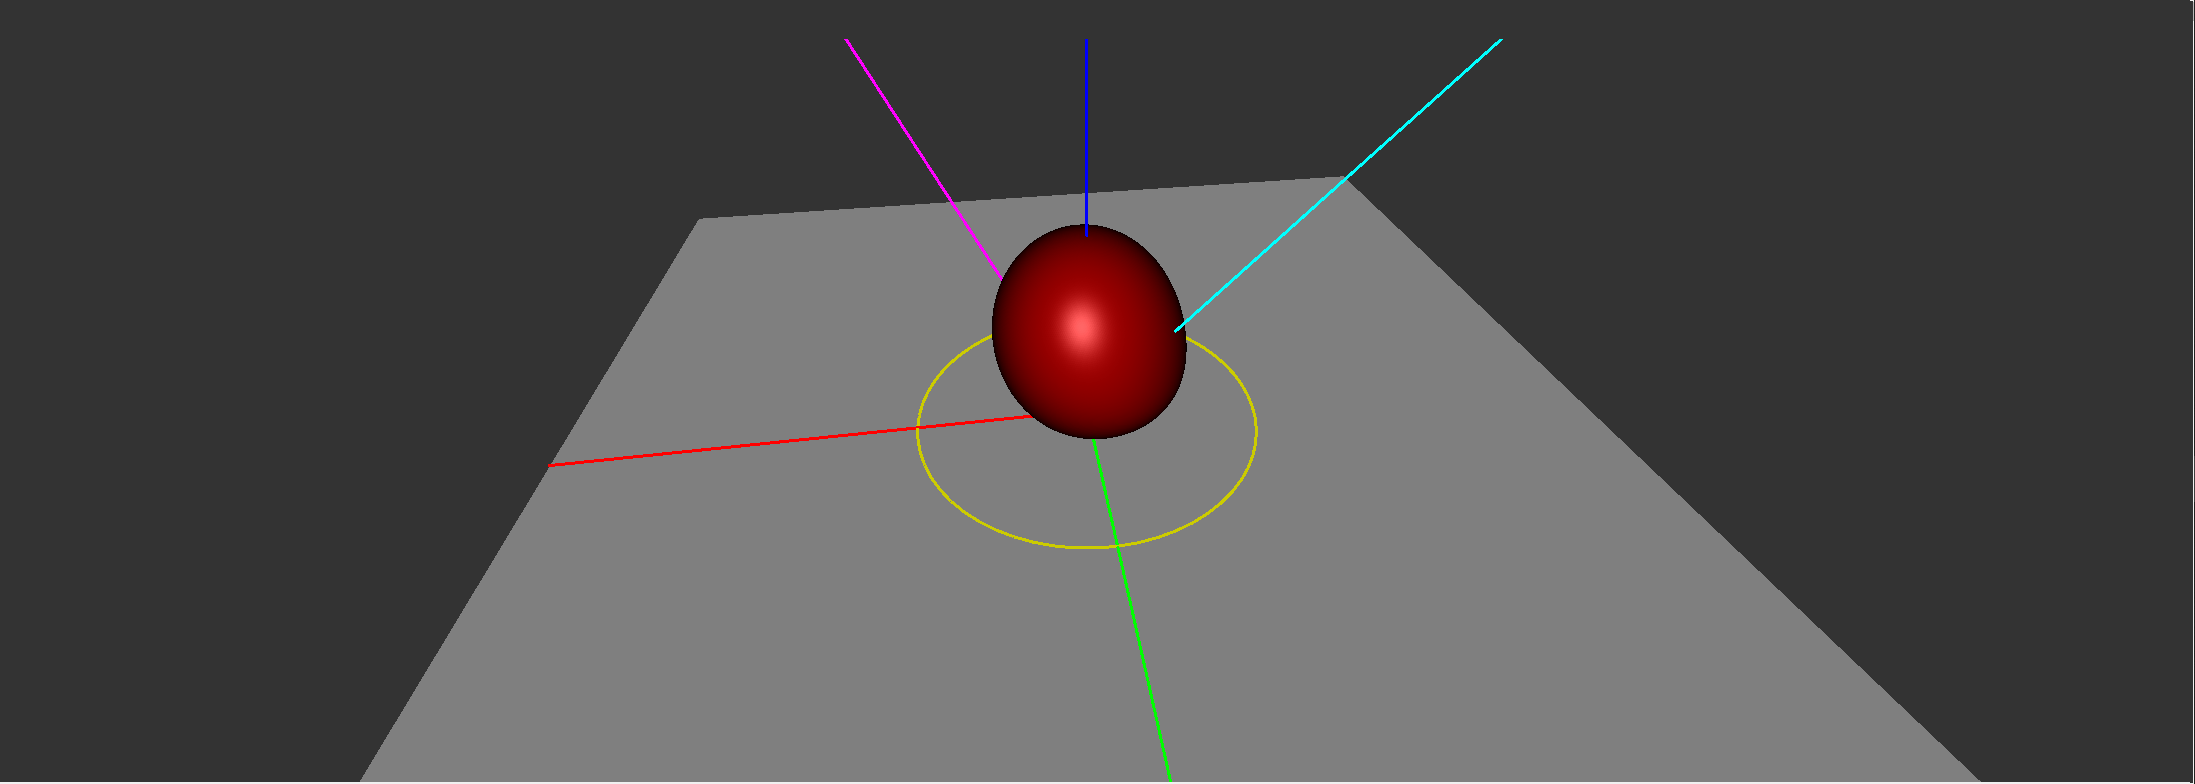
\includegraphics[width=\linewidth]{./Imagens/brdfs/edwards-2006-3D-plot}
    % \vspace{0.1px}
    \legend{ \small (a) 3D \textit{plot}}
\endminipage\hfill
\minipage{0.48\textwidth}
  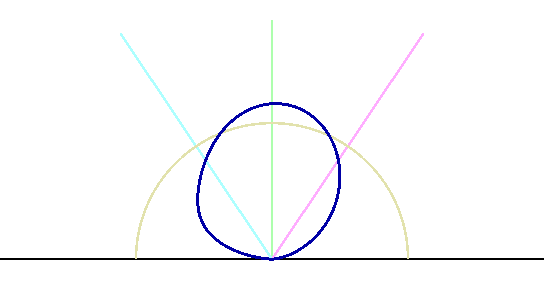
\includegraphics[width=\linewidth]{./Imagens/brdfs/edwards-2006-polar-plot.png}
    \legend{ \small (b) \textit{Polar plot}}
\endminipage\hfill
\end{figure}

\begin{figure}[H]
    \caption{\small{Objetos 3D renderizados pelo experimento Edwards.}}\label{fig-edwards-2006-eqlang}
\minipage{0.32\textwidth}
  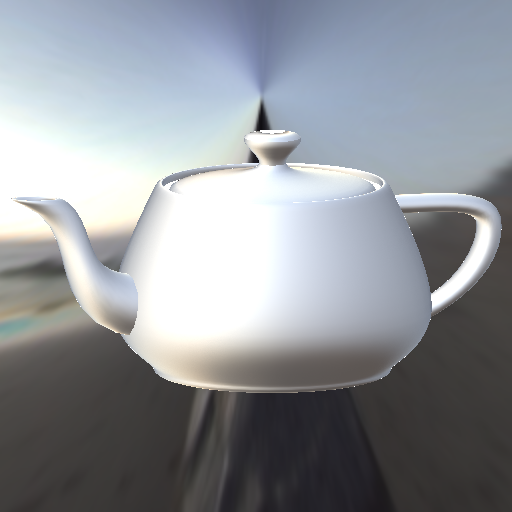
\includegraphics[width=\linewidth]{./Imagens/brdfs/edwards-2006-teapot.png}
    \legend{ \small (a) \textit{Teapot}}
\endminipage\hfill
\minipage{0.32\textwidth}
  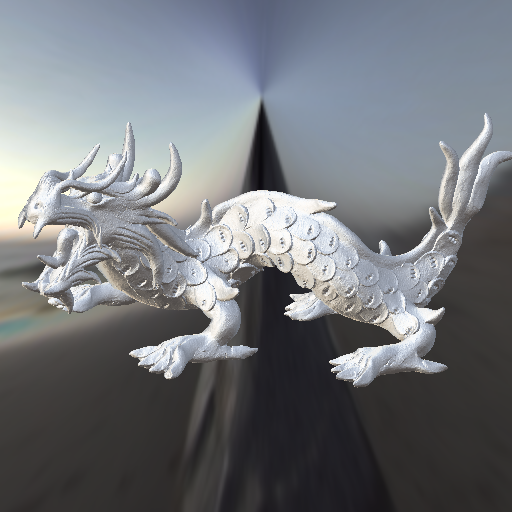
\includegraphics[width=\linewidth]{./Imagens/brdfs/edwards-2006-dragon.png}
    \legend{ \small (b) Dragão de Stanford}
\endminipage\hfill
\minipage{0.32\textwidth}%
  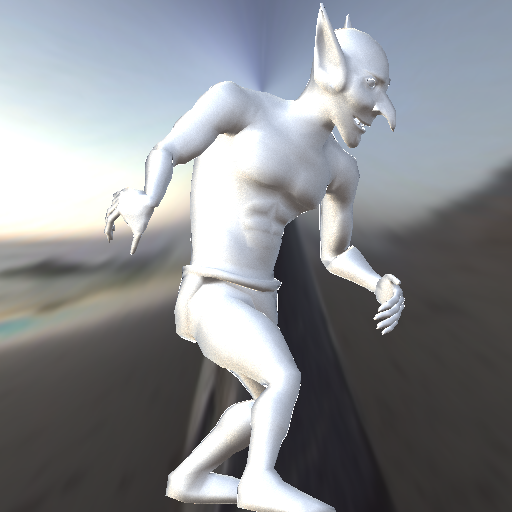
\includegraphics[width=\linewidth]{./Imagens/brdfs/edwards-2006-goblin.png}
    \legend{ \small (c) Goblin}
\endminipage
\end{figure}

